\chapter{Insiemi Ordinati, Reticoli e Strutture Booleane}
\label{chap:ordini_reticoli}

Lo studio delle relazioni d'ordine parziale e dei reticoli costituisce uno dei temi più ricorrenti e qualificanti delle prove scritte e dei colloqui orali con il Prof. Cutolo. In questo capitolo sviluppiamo la teoria a partire dai diagrammi di Hasse fino al teorema di Stone per le algebre di Boole finite.

\section{Insiemi Parzialmente Ordinati (Poset)}

\begin{definizione}{Relazione d'Ordine}{rel_ordine}
Una relazione binaria $\le$ su un insieme $P$ è detta \textbf{relazione d'ordine parziale (largo)} se soddisfa:
\begin{enumerate}
    \item \textbf{Riflessività:} $\forall x \in P, x \le x$;
    \item \textbf{Antisimmetria:} $\forall x, y \in P, (x \le y \wedge y \le x) \implica x = y$;
    \item \textbf{Transitività:} $\forall x, y, z \in P, (x \le y \wedge y \le z) \implica x \le z$.
\end{enumerate}
La coppia $(P, \le)$ è detta \textbf{insieme parzialmente ordinato} (o \textbf{poset}, dall'inglese \emph{partially ordered set}).

L'ordine si dice \textbf{totale} (o lineare) se ogni coppia di elementi è confrontabile:
\[
    \forall x, y \in P, \quad x \le y \vee y \le x
\]
In tal caso, il poset è detto \textbf{catena}.
\end{definizione}

\subsection{Principio di Dualità per Poset}
Data una relazione d'ordine $\le$ su $P$, la relazione inversa $\ge$ (definita da $x \ge y \iff y \le x$) è anch'essa una relazione d'ordine parziale su $P$, detta \textbf{ordine duale}.
Ne discende il \textbf{Principio di Dualità}: ogni teorema valido per una relazione d'ordine $\le$ rimane valido sostituendo simultaneamente ogni occorrenza di $\le$ con $\ge$ (e scambiando i concetti duali: minimo con massimo, $\inf$ con $\sup$, minoranti con maggioranti).

\section{Elementi Speciali in un Poset}

Sia $(P, \le)$ un poset e sia $S \sseq P$.

\begin{definizione}{Minimo, Massimo, Minimali e Massimali}{elementi_speciali}
Sia $m \in P$:
\begin{itemize}
    \item $m$ è il \textbf{minimo} di $P$ ($m = \min(P)$) se:
    \[
        \forall x \in P, \quad m \le x
    \]
    \item $M$ è il \textbf{massimo} di $P$ ($M = \max(P)$) se:
    \[
        \forall x \in P, \quad x \le M
    \]
    \item $u \in P$ è un \textbf{elemento minimale} se nessun elemento di $P$ è strettamente minore di $u$:
    \[
        \forall x \in P, \quad x \le u \Implica x = u
    \]
    \item $v \in P$ è un \textbf{elemento massimale} se nessun elemento di $P$ è strettamente maggiore di $v$:
    \[
        \forall x \in P, \quad v \le x \Implica x = v
    \]
\end{itemize}
\end{definizione}

\begin{proposizione}{Unicità del Minimo e del Massimo}{unicita_min_max}
In qualunque poset $(P, \le)$, se il minimo (risp. massimo) esiste, esso è \textbf{unico}.
\end{proposizione}
\begin{proof}
Siano $m_1, m_2$ due minimi di $P$. Essendo $m_1$ un minimo e $m_2 \in P$, si ha $m_1 \le m_2$. Essendo $m_2$ un minimo e $m_1 \in P$, si ha $m_2 \le m_1$. Per l'antisimmetria della relazione d'ordine, $m_1 = m_2$.
\end{proof}

\begin{avvisoCutolo}
    \textbf{Minimo vs Elemento Minimale: Una Distinzione Cruciale!}
    \begin{itemize}
        \item Se un poset possiede un \textbf{minimo} $m$, allora $m$ è anche l'\textbf{unico elemento minimale} di $P$.
        \item Il viceversa è falso in generale per insiemi infiniti, ma è vero se il poset è finito ed esiste un solo minimale.
        \item Un poset può non avere minimo e possedere \textbf{molteplici elementi minimali} (in tal caso reciprocamente non confrontabili), oppure non averne alcuno.
    \end{itemize}
\end{avvisoCutolo}

\begin{teorema}{Esistenza di Minimali e Massimali in Poset Finiti}{teo_esist_finiti}
Ogni poset finito non vuoto $(P, \le)$ ammette \textbf{almeno un elemento minimale} e \textbf{almeno un elemento massimale}.
\end{teorema}

\subsection{Minoranti, Maggioranti, Estremo Inferiore ed Estremo Superiore}

Sia $(P, \le)$ un poset e sia $S \sseq P$:
\begin{itemize}
    \item L'insieme dei \textbf{minoranti} di $S$ è $\minor(S) = \{x \in P \mid \forall s \in S, x \le s\}$.
    \item L'insieme dei \textbf{maggioranti} di $S$ è $\maggior(S) = \{x \in P \mid \forall s \in S, s \le x\}$.
    \item Se $\minor(S)$ ammette massimo in $P$, tale massimo è detto \textbf{estremo inferiore} di $S$ e si indica con $\inf(S)$ o $\bigwedge S$:
    \[
        \inf(S) = \max(\minor(S))
    \]
    \item Se $\maggior(S)$ ammette minimo in $P$, tale minimo è detto \textbf{estremo superiore} di $S$ e si indica con $\sup(S)$ o $\bigvee S$:
    \[
        \sup(S) = \min(\maggior(S))
    \]
\end{itemize}

Nel caso di una coppia $S = \{a, b\}$, si usa la notazione $a \wedge b = \inf(a, b)$ e $a \vee b = \sup(a, b)$.

\section{Relazione di Copertura e Diagrammi di Hasse}

Nei poset finiti, gran parte della relazione d'ordine è ridondante a causa delle proprietà riflessiva e transitiva. La struttura essenziale è catturata dalla relazione di copertura.

\begin{definizione}{Relazione di Copertura}{copertura}
Dati due elementi $x, y \in P$, si dice che $y$ \textbf{copre} $x$ (e si scrive $x \prec y$) se:
\[
    x < y \quad \wedge \quad \neg(\exists z \in P : x < z < y)
\]
ovvero se non esiste alcun elemento intermedio strettamente compreso tra $x$ e $y$.
\end{definizione}

\begin{definizione}{Diagramma di Hasse}{hasse}
Il \textbf{diagramma di Hasse} di un poset finito $(P, \le)$ è una rappresentazione grafica planare in cui:
\begin{enumerate}
    \item Gli elementi di $P$ sono rappresentati da punti (o nodi) nel piano;
    \item Se $x \prec y$, il nodo $y$ è collocato a un'altezza verticale superiore rispetto a $x$;
    \item Un segmento congiunge $x$ e $y$ se e solo se $y$ copre $x$ ($x \prec y$).
\end{enumerate}
\end{definizione}

Per risalire alla relazione d'ordine a partire dal diagramma: $a \le b$ se e solo se $a = b$ oppure esiste un cammino ascendente di segmenti che sale da $a$ fino a $b$.

\begin{figure}[htbp]
\centering
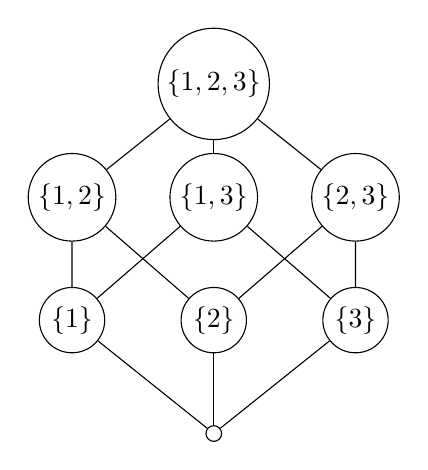
\begin{tikzpicture}[scale=1.2, every node/.style={circle, draw, fill=white, inner sep=2pt}]
    % Diagramma di Hasse per P({1,2,3})
    \node (0) at (0, 0) {$\vuoto$};
    \node (1) at (-1.5, 1.2) {$\{1\}$};
    \node (2) at (0, 1.2) {$\{2\}$};
    \node (3) at (1.5, 1.2) {$\{3\}$};
    \node (12) at (-1.5, 2.5) {$\{1,2\}$};
    \node (13) at (0, 2.5) {$\{1,3\}$};
    \node (23) at (1.5, 2.5) {$\{2,3\}$};
    \node (123) at (0, 3.7) {$\{1,2,3\}$};
    
    \draw (0) -- (1); \draw (0) -- (2); \draw (0) -- (3);
    \draw (1) -- (12); \draw (1) -- (13);
    \draw (2) -- (12); \draw (2) -- (23);
    \draw (3) -- (13); \draw (3) -- (23);
    \draw (12) -- (123); \draw (13) -- (123); \draw (23) -- (123);
\end{tikzpicture}
\caption{Diagramma di Hasse del reticolo booleano $(\P(\{1,2,3\}), \sseq)$.}
\label{fig:hasse_p3}
\end{figure}

\section{Reticoli: Definizione d'Ordine ed Algebrica}

\begin{definizione}{Reticolo (come Poset)}{reticolo_poset}
Un poset $(L, \le)$ si dice \textbf{reticolo} se per ogni coppia di elementi $a, b \in L$ esistono in $L$ sia l'estremo inferiore che l'estremo superiore:
\[
    \forall a, b \in L, \quad \exists (a \wedge b) = \inf(a, b) \quad \wedge \quad \exists (a \vee b) = \sup(a, b)
\]
\end{definizione}

\begin{definizione}{Reticolo (come Struttura Algebrica)}{reticolo_alg}
Una struttura algebrica $(L, \wedge, \vee)$ dotata di due operazioni binarie interne si dice \textbf{reticolo} se per ogni $a, b, c \in L$ sono soddisfatti i seguenti assiomi:
\begin{enumerate}
    \item \textbf{Commutatività:} $a \wedge b = b \wedge a$, \quad $a \vee b = b \vee a$;
    \item \textbf{Associatività:} $(a \wedge b) \wedge c = a \wedge (b \wedge c)$, \quad $(a \vee b) \vee c = a \vee (b \vee c)$;
    \item \textbf{Idempotenza:} $a \wedge a = a$, \quad $a \vee a = a$;
    \item \textbf{Leggi di Assorbimento:} $a \wedge (a \vee b) = a$, \quad $a \vee (a \wedge b) = a$.
\end{enumerate}
\end{definizione}

\begin{teorema}{Teorema di Equivalenza tra le Definizioni di Reticolo}{teo_equiv_reticolo}
Le nozioni di reticolo come poset e di reticolo come struttura algebrica sono \textbf{perfettamente equivalenti}:
\begin{enumerate}
    \item Se $(L, \le)$ è un reticolo d'ordine, ponendo $a \wedge b = \inf(a, b)$ e $a \vee b = \sup(a, b)$, la struttura $(L, \wedge, \vee)$ soddisfa i 4 assiomi algebrici.
    \item Viceversa, se $(L, \wedge, \vee)$ è un reticolo algebrico, la relazione binaria definita su $L$ da:
    \[
        a \le b \quad \Shiff \quad a \wedge b = a \quad \Shiff \quad a \vee b = b
    \]
    è una relazione d'ordine parziale su $L$ tale che $\inf(a, b) = a \wedge b$ e $\sup(a, b) = a \vee b$.
\end{enumerate}
\end{teorema}

\begin{avvisoCutolo}
    \textbf{Dimostrazione Obbligatoria all'Orale: L'Associatività di $\inf$!}
    Il Prof. Cutolo chiede sistematicamente la dimostrazione formale che $\inf$ è associativo \textbf{lavorando unicamente con la definizione d'ordine di estremo inferiore}, senza assumere a priori l'assioma algebrico!
\end{avvisoCutolo}

\begin{proof}[Dimostrazione che $\inf$ è associativo in un poset]
Sia $(L, \le)$ un reticolo d'ordine e siano $a, b, c \in L$.
Poniamo $d_1 = a \wedge (b \wedge c)$ e $d_2 = (a \wedge b) \wedge c$. Vogliamo dimostrare che $d_1 = d_2$.
Mostriamo anzitutto che $d_1 = \inf(\{a, b, c\})$.
Per definizione di estremo inferiore:
\begin{enumerate}
    \item $d_1 = \inf(a, b \wedge c) \implies d_1 \le a$ e $d_1 \le (b \wedge c)$.
    \item A sua volta, $d_1 \le (b \wedge c) \implies d_1 \le b$ e $d_1 \le c$.
    Dunque $d_1$ è un minorante comune di $\{a, b, c\}$, cioè $d_1 \in \minor(\{a, b, c\})$.
    \item Sia ora $x \in L$ un qualunque minorante comune di $\{a, b, c\}$, ovvero $x \le a$, $x \le b$ e $x \le c$.
    Poiché $x \le b$ e $x \le c$, per la proprietà di massimo dei minoranti si ha $x \le \inf(b, c) = b \wedge c$.
    Ora abbiamo $x \le a$ e $x \le (b \wedge c)$. Di conseguenza, $x \le \inf(a, b \wedge c) = d_1$.
\end{enumerate}
Ciò prova che $d_1$ è il massimo dei minoranti di $\{a, b, c\}$, cioè $d_1 = \inf(\{a, b, c\})$.
Ripetendo lo stesso identico ragionamento per $d_2 = (a \wedge b) \wedge c$, si ottiene che anch'esso è l'estremo inferiore di $\{a, b, c\}$.
Poiché per la Proposizione~\ref{prop:unicita_min_max} l'estremo inferiore (essendo un massimo) è unico se esiste, si conclude che $d_1 = d_2$.
\end{proof}

\subsection{Reticoli Limitati e Reticoli Completi}
Un reticolo $(L, \wedge, \vee)$ si dice:
\begin{itemize}
    \item \textbf{Limitato} se possiede sia elemento minimo $0 = \min(L)$ che massimo $1 = \max(L)$. In tal caso:
    \[
        \forall x \in L, \quad x \wedge 0 = 0, \quad x \vee 0 = x, \quad x \wedge 1 = x, \quad x \vee 1 = 1
    \]
    Ogni reticolo finito non vuoto è limitato: $0 = \bigwedge L$ e $1 = \bigvee L$.
    \item \textbf{Completo} se ogni sottoinsieme non vuoto $S \sseq L$ (anche infinito) ammette estremo inferiore e superiore in $L$.
\end{itemize}

\section{Reticoli Distributivi e Criterio di Birkhoff}

\begin{definizione}{Reticolo Distributivo}{ret_distributivo}
Un reticolo $(L, \wedge, \vee)$ si dice \textbf{distributivo} se l'operazione $\wedge$ si distribuisce su $\vee$:
\[
    \forall a, b, c \in L, \quad a \wedge (b \vee c) = (a \wedge b) \vee (a \wedge c)
\]
In ogni reticolo, la validità di questa identità è \textbf{equivalente} alla validità della legge distributiva duale:
\[
    a \vee (b \wedge c) = (a \vee b) \wedge (a \vee c)
\]
\end{definizione}

In ogni reticolo vale sempre la disuguaglianza distributiva:
\[
    (a \wedge b) \vee (a \wedge c) \le a \wedge (b \vee c)
\]
Nei reticoli non distributivi tale disuguaglianza può essere stretta.

\begin{teorema}{Criterio di Distributività di Birkhoff}{birkhoff}
Un reticolo $L$ è distributivo \textbf{se e solo se} non contiene alcun sottoreticolo isomorfo al \textbf{pentagono} $N_5$ o al \textbf{diamante} $M_3$.
\end{teorema}

\begin{figure}[htbp]
\centering
\begin{minipage}{0.45\textwidth}
\centering
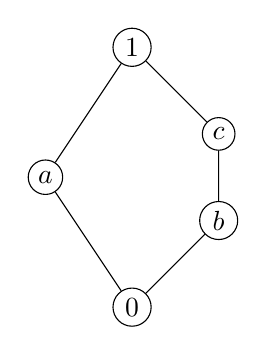
\begin{tikzpicture}[scale=1.1, every node/.style={circle, draw, fill=white, inner sep=2pt}]
    \node (0) at (0, 0) {$0$};
    \node (a) at (-1, 1.5) {$a$};
    \node (b) at (1, 1) {$b$};
    \node (c) at (1, 2) {$c$};
    \node (1) at (0, 3) {$1$};
    \draw (0) -- (a) -- (1);
    \draw (0) -- (b) -- (c) -- (1);
\end{tikzpicture}
\caption*{Pentagono $N_5$ (Non modulare)}
\end{minipage}
\hfill
\begin{minipage}{0.45\textwidth}
\centering
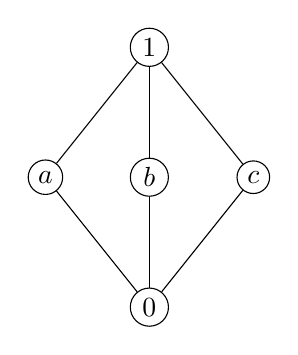
\begin{tikzpicture}[scale=1.1, every node/.style={circle, draw, fill=white, inner sep=2pt}]
    \node (0) at (0, 0) {$0$};
    \node (a) at (-1.2, 1.5) {$a$};
    \node (b) at (0, 1.5) {$b$};
    \node (c) at (1.2, 1.5) {$c$};
    \node (1) at (0, 3) {$1$};
    \draw (0) -- (a) -- (1);
    \draw (0) -- (b) -- (1);
    \draw (0) -- (c) -- (1);
\end{tikzpicture}
\caption*{Diamante $M_3$ (Modulare non distributivo)}
\end{minipage}
\caption{I due reticoli proibiti del Criterio di Birkhoff.}
\label{fig:n5_m3}
\end{figure}

\begin{avvisoCutolo}
    Nel pentagono $N_5$, si osservi che $b < c$, ma:
    \[
        a \wedge (b \vee c) = a \wedge 1 = a \neq b = b \vee 0 = (a \wedge b) \vee (a \wedge c)
    \]
    Nel diamante $M_3$:
    \[
        a \wedge (b \vee c) = a \wedge 1 = a \neq 0 = 0 \vee 0 = (a \wedge b) \vee (a \wedge c)
    \]
    All'orale o nello scritto, per dimostrare che un reticolo non è distributivo, basta esibire una terna di elementi che viola la legge distributiva!
\end{avvisoCutolo}

\section{Complementi, Algebre di Boole e Anelli Booleani}

\begin{definizione}{Complemento e Reticolo Complementato}{complemento}
Sia $(L, \wedge, \vee, 0, 1)$ un reticolo limitato. Sia $a \in L$. Un elemento $b \in L$ si dice \textbf{complemento} di $a$ se:
\[
    a \wedge b = 0 \quad \wedge \quad a \vee b = 1
\]
Un reticolo limitato in cui \textbf{ogni elemento ammette almeno un complemento} si dice \textbf{reticolo complementato}.
\end{definizione}

\begin{teorema}{Unicità del Complemento nei Reticoli Distributivi}{unicita_comp}
Sia $L$ un reticolo \textbf{distributivo} limitato. Se un elemento $a \in L$ ammette un complemento, questo è \textbf{unico}.
\end{teorema}
\begin{proof}
Siano $b_1, b_2$ due complementi di $a$, dunque $a \wedge b_1 = 0$, $a \vee b_1 = 1$, $a \wedge b_2 = 0$, $a \vee b_2 = 1$.
Calcoliamo:
\[
    b_1 = b_1 \wedge 1 = b_1 \wedge (a \vee b_2) = (b_1 \wedge a) \vee (b_1 \wedge b_2) = 0 \vee (b_1 \wedge b_2) = b_1 \wedge b_2
\]
Dunque $b_1 \le b_2$. Scambiando i ruoli di $b_1$ e $b_2$, si ottiene analogamente $b_2 \le b_1$. Per antisimmetria, $b_1 = b_2$.
\end{proof}

\begin{definizione}{Reticolo Booleano e Algebra di Boole}{boole}
Un reticolo si dice \textbf{booleano} se è distributivo e complementato.
L'unico complemento di $a$ si denota con $a'$ (oppure $\neg a$ o $\bar{a}$).
La struttura $(B, \wedge, \vee, ', 0, 1)$ è detta \textbf{algebra di Boole}.
\end{definizione}

Nelle algebre di Boole valgono le leggi di De Morgan per il complemento:
\[
    (a \wedge b)' = a' \vee b', \qquad (a \vee b)' = a' \wedge b'
\]

\begin{teorema}{Teorema di Stone per Algebre di Boole Finite}{stone}
Ogni algebra di Boole finita $B$ è isomorfa al reticolo delle parti $(\P(S), \cap, \cup)$ dell'insieme dei suoi atomi $S = \operatorname{Atomi}(B)$.
In particolare, la cardinalità di ogni algebra di Boole finita è una \textbf{potenza di 2}:
\[
    |B| = 2^n \quad (\text{con } n = |S|)
\]
\end{teorema}

\begin{definizione}{Anello Booleano}{anello_boole}
Un anello $(R, +, \cdot)$ con unità si dice \textbf{anello booleano} se ogni suo elemento è \textbf{idempotente}:
\[
    \forall x \in R, \quad x^2 = x
\]
\end{definizione}

\begin{teorema}{Proprietà degli Anelli Booleani}{prop_anelli_boole}
Sia $R$ un anello booleano. Allora:
\begin{enumerate}
    \item $R$ ha caratteristica 2: per ogni $x \in R$, $x + x = 0$ (ovvero $x = -x$);
    \item $R$ è commutativo: per ogni $x, y \in R$, $xy = yx$.
\end{enumerate}
\end{teorema}
\begin{proof}
1. Consideriamo $(x + x)^2 = x + x$. Per distributività, $(x+x)^2 = x^2 + x^2 + x^2 + x^2 = x + x + x + x$. Uguagliando: $x + x + x + x = x + x \implies x + x = 0$.
2. Consideriamo $(x + y)^2 = x + y$. Espandendo: $x^2 + xy + yx + y^2 = x + xy + yx + y$. Poiché $x^2 = x$ e $y^2 = y$, otteniamo $xy + yx = 0$. Essendo $yx = -yx$, si ha $xy = -yx = yx$.
\end{proof}

\begin{teorema}{Equivalenza tra Algebre di Boole e Anelli Booleani}{equiv_boole}
Ogni algebra di Boole $(B, \wedge, \vee, ', 0, 1)$ diviene un anello booleano ponendo:
\[
    a + b \coloneqq (a \wedge b') \vee (a' \wedge b) = a \ds b, \qquad a \cdot b \coloneqq a \wedge b
\]
Viceversa, ogni anello booleano unitario $(R, +, \cdot)$ diviene un'algebra di Boole ponendo:
\[
    a \wedge b \coloneqq a \cdot b, \qquad a \vee b \coloneqq a + b + ab, \qquad a' \coloneqq 1 + a
\]
\end{teorema}
